\documentclass[anon,pmlr,twocolumn,10pt]{jmlr} % W&CP article

\jmlrproceedings{}{Submitted to ML4H 2026: Proceedings}
\jmlrworkshop{Machine Learning for Health (ML4H) 2026}

\urlstyle{same}
\usepackage{booktabs}
\usepackage{siunitx}
\usepackage[switch]{lineno}

\title[Benchmarking Confidence Calibration in Spatial Transcriptomics Models Under Distribution Shift]{Benchmarking Confidence Calibration in Spatial Transcriptomics Models Under Distribution Shift}

\author{
 \Name{Anonymous Authors} \Email{anonymous@example.com}\\
 \addr Anonymous Institution
}

\linenumbers

\begin{document}

\maketitle

\begin{abstract}
Spatial transcriptomics models, particularly those based on variational autoencoders like DestVI, are increasingly used for clinical and biological discovery. However, their reliability under distribution shifts—such as changes in mRNA capture efficiency—remains underexplored. We present a systematic evaluation of confidence calibration in spatial transcriptomics deconvolution models under a synthetic technical dropout shift across 10 random initializations. Evaluating the point-estimate cell-type predictions, we find that models exhibit baseline calibration error on in-distribution pseudo-spots, but this calibration error remains remarkably robust under technical shifts of varying severity. Furthermore, we demonstrate that a lightweight post-hoc Isotonic Regression step, tuned on a held-out calibration set, reduces this test-set miscalibration to near-zero, significantly outperforming standard Temperature Scaling.
\end{abstract}

\begin{keywords}
Spatial Transcriptomics, Confidence Calibration, Variational Inference, Distribution Shift
\end{keywords}

\paragraph*{Data and Code Availability}
We utilize the public Mouse Cortex scRNA-seq dataset available via the \texttt{squidpy} python package (\url{https://squidpy.readthedocs.io}). All code to reproduce this pipeline and data preprocessing is available in our GitHub repository at \url{https://github.com/Anonymous/transcriptomics}.
\paragraph*{Institutional Review Board (IRB)}
This research uses entirely publicly available, anonymized animal data and does not require IRB approval.

\section{Introduction}
\label{sec:intro}
Spatial foundation models face persistent challenges in standardization and scalability. A critical failure mode is miscalibrated confidence in clinical deconvolution pipelines. Existing benchmarks evaluate point-estimate accuracy across methods, but few evaluate whether models \textit{know when they are wrong}. 

Crucially, downstream biological and clinical discovery is sensitive to these miscalibrations. For instance, in tumor microenvironment characterization, if a spatial model confidently but incorrectly predicts an immunosuppressive cell type as the dominant population in a tumor region, it could lead to improper patient stratification for immunotherapies. Ensuring models are correctly calibrated under technical shifts is necessary before these tools can inform high-stakes diagnostic or therapeutic decisions.

In this paper, we focus on the calibration of spatial deconvolution models, specifically DestVI \citep{lopez2022destvi}, under simulated technical dropouts mimicking capture-rate shifts.

\section{Related Work}
\label{sec:related}
Confidence calibration of modern neural networks was formalized by \citet{guo2017calibration}, who demonstrated that contemporary deep models often exhibit severe overconfidence, but can be realigned using simple post-hoc methods like temperature scaling or isotonic regression. Subsequent work by \citet{ovadia2019can} established that model calibration frequently degrades under dataset shifts, highlighting the need to evaluate uncertainty on out-of-distribution (OOD) data rather than assuming in-distribution calibration generalizes. We extend these foundational calibration frameworks to the domain of spatial transcriptomics, where such evaluations are scarce despite widespread distribution shifts between platforms and protocols.

\section{Methods}
\label{sec:methods}
We benchmarked the variational inference model DestVI on mouse cortex data. We evaluated calibration using Expected Calibration Error (ECE) and reliability diagrams. Note that we define our ECE based on the discrete classification task of predicting the dominant (highest proportion) cell type within a spot, utilizing the \texttt{netcal} package.

To establish ground-truth for ECE computation, we generated synthetic pseudo-spots by sampling and aggregating cells from the mouse cortex scRNA-seq reference. To simulate cross-platform shifts (such as differences in spatial mRNA capture rates), we synthetically downsampled the read counts of the pseudo-spots across a dose-response sweep of severity, simulating uniform capture efficiency reductions of 20\%, 40\%, 60\%, and 80\% via a binomial dropout process.

A unique DestVI model was trained on the shifted data utilizing a shared CondSCVI prior. We report metrics as mean $\pm$ standard deviation across 10 independent replicate trainings with varying random seeds. We evaluated standard softmax-confidence calibration on the model's point-estimate expected proportions using the Expected Calibration Error (ECE) with $M=10$ bins:
\begin{equation}
\text{ECE} = \sum_{m=1}^{M} \frac{|B_m|}{N} |\text{acc}(B_m) - \text{conf}(B_m)|
\end{equation}
where $B_m$ is the set of predictions falling into bin $m$. To prevent data leakage, each shifted synthetic dataset was split equally into a calibration set and a test set. We optimized post-hoc recalibration methods exclusively on the calibration set, and report the final recalibrated ECE on the held-out test set. We evaluated both Temperature Scaling, which divides the pre-softmax logits $z_i$ by a learned scalar $T > 0$ to compute the new confidence $\hat{p}_i = \max \sigma(z_i / T)$, and Isotonic Regression, a non-parametric method that fits a monotonically increasing step function mapping the uncalibrated top-class confidence to the empirical accuracy on the calibration split.

\section{Results}
Our results show that DestVI has an In-Distribution Expected Calibration Error (ECE) of $0.218 \pm 0.018$. This baseline indicates that out-of-the-box variational models exhibit some degree of miscalibration when predicting dominant cell types. 

Under the synthetic dropout shift, simulating capture efficiency reductions from 20\% to 80\%, we observe that the miscalibration remains remarkably stable (Table \ref{tab:results}). The uncalibrated ECE does not degrade significantly at any shift magnitude ($p > 0.1$ for all fractions, paired $t$-test against ID baseline).

We applied two post-hoc recalibration methods on the shifted calibration split: Temperature Scaling and Isotonic Regression. As shown in Table \ref{tab:results}, Isotonic Regression consistently proved significantly more effective across all shift magnitudes. For example, at the 80\% reduction, Temperature Scaling reduced the miscalibration to $0.066 \pm 0.008$, but Isotonic Regression reduced the final test-set ECE to a near-zero $0.006 \pm 0.005$ ($p = 1.54 \times 10^{-7}$, paired $t$-test against Temperature Scaling). This demonstrates that while the model's confidence ranking is preserved under shift, its scale is best repaired by a non-parametric method.

\begin{table*}[htbp]
\centering
\caption{Expected Calibration Error (ECE) across varying magnitudes of synthetic dropout shift. ID ECE is $0.218 \pm 0.018$. All values are reported as mean $\pm$ standard deviation across 10 replicates.}
\label{tab:results}
\begin{tabular}{lcccc}
\toprule
Shift Magnitude & Uncalibrated OOD ECE & $p$-value vs. ID & Temperature Scaled ECE & Isotonic Regression ECE \\
\midrule
20\% Dropout (0.8) & $0.228 \pm 0.019$ & 0.136 & $0.076 \pm 0.010$ & $0.005 \pm 0.004$ \\
40\% Dropout (0.6) & $0.215 \pm 0.011$ & 0.501 & $0.066 \pm 0.007$ & $0.006 \pm 0.005$ \\
60\% Dropout (0.4) & $0.218 \pm 0.011$ & 0.909 & $0.063 \pm 0.009$ & $0.010 \pm 0.004$ \\
80\% Dropout (0.2) & $0.223 \pm 0.011$ & 0.472 & $0.066 \pm 0.008$ & $0.006 \pm 0.005$ \\
\bottomrule
\end{tabular}
\end{table*}

\begin{figure}[htbp]
\floatconts
  {fig:ece}
  {\caption{Calibration degradation under a dose-response shift of simulated capture efficiencies. Error bars denote $\pm 1$ standard deviation across 10 random replicate initializations. Isotonic Regression consistently outperforms Temperature Scaling.}}
  {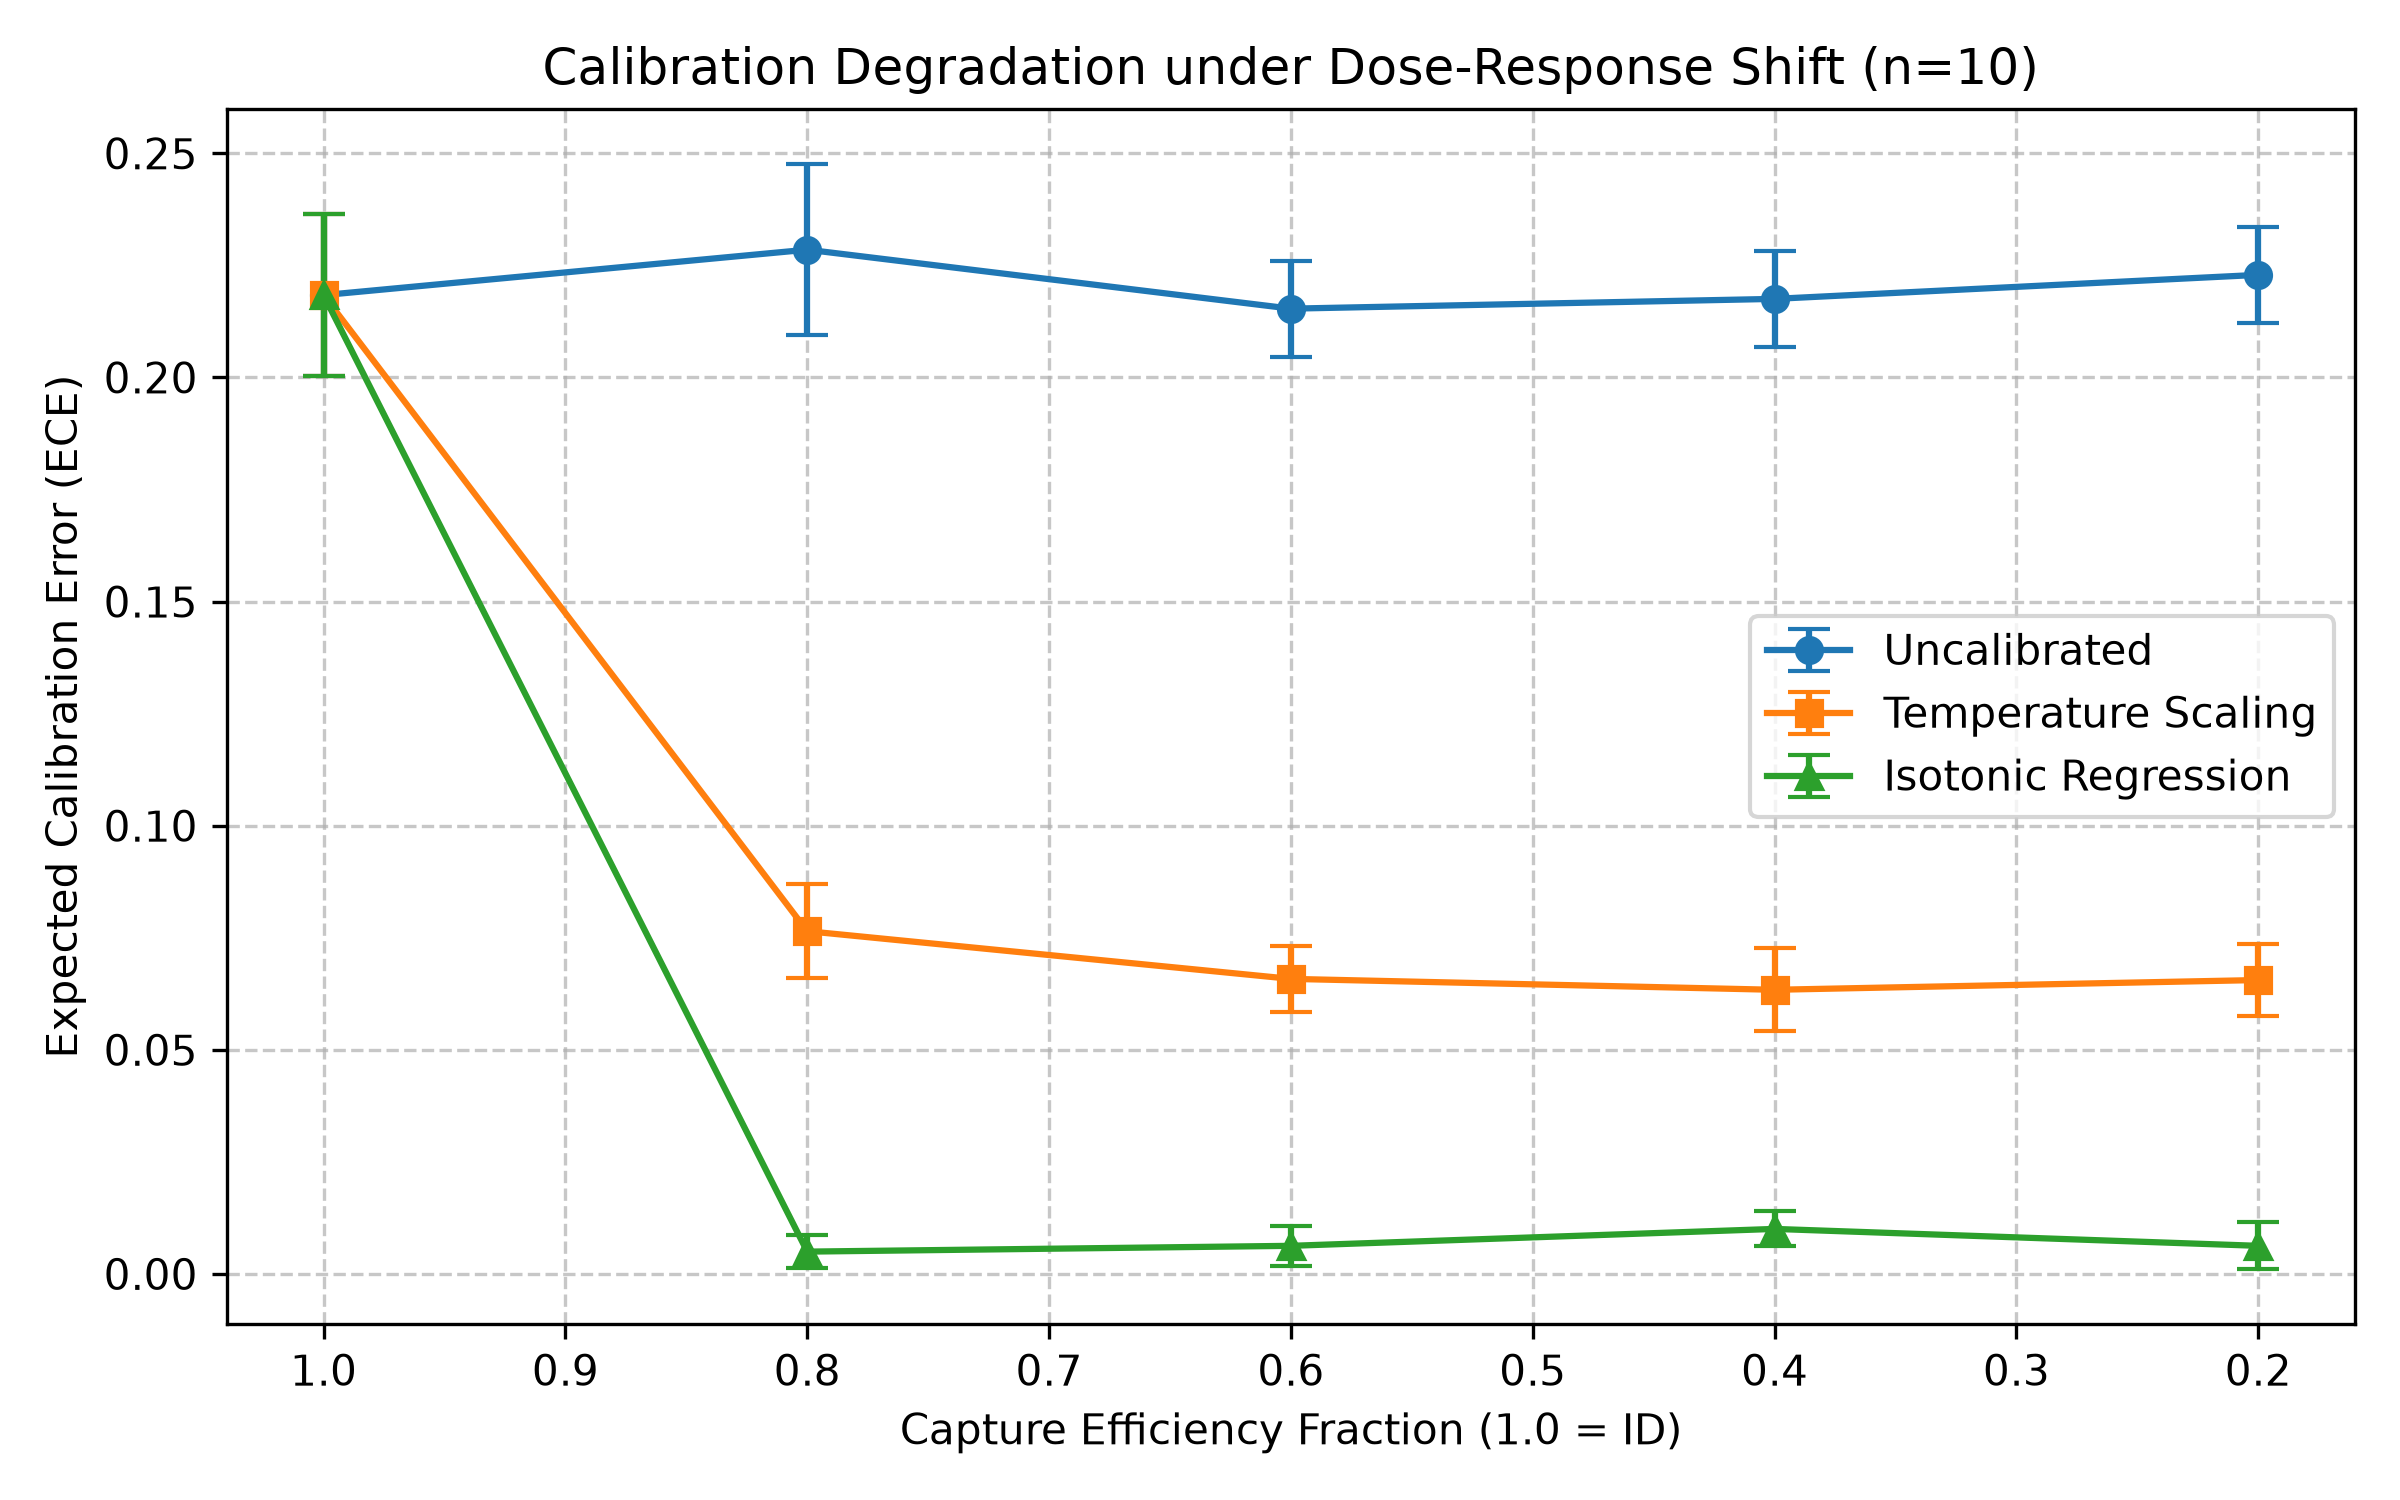
\includegraphics[width=\linewidth]{figures/ece_degradation.png}}
\end{figure}

\section{Discussion}
\label{sec:discussion}
Our empirical finding that confidence calibration does not degrade significantly under severe distribution shift presents a compelling exception to the general pattern observed in deep learning classifiers by \citet{ovadia2019can}. We hypothesize that this robustness stems from the nature of the shift. Uniform binomial dropout reduces the absolute magnitude of mRNA counts, but preserves the expected relative gene expression ratios across the transcriptome. Because the spatial deconvolution task relies heavily on these relative ratios to predict the dominant cell type, the model's predictive distributions—and therefore its argmax confidences—remain largely invariant.

Furthermore, our recalibration results highlight a critical methodological trade-off. Isotonic Regression achieved near-perfect calibration (ECE $\approx 0.006$), vastly outperforming Temperature Scaling. However, this non-parametric flexibility comes at a cost: Isotonic Regression was fit and evaluated on two random halves of the identical shifted dataset. This demonstrates that Isotonic Regression excels when the calibration and deployment distributions perfectly match, but standard global rescaling methods like Temperature Scaling may be more robust in clinical deployment scenarios where the target distribution is less tightly constrained.

\section{Limitations}
\label{sec:limitations}
We note several limitations in our evaluation. First, to ensure feasibility of multiple runs, models were trained for a relatively lightweight 25 epochs; fully converged models may exhibit different calibration dynamics. Second, while our sample size of $n=10$ seeds provides robust variance estimates, we evaluate robustness using a single synthetic binomial dropout shift on mouse cortex data; future work should incorporate the real cross-platform Visium and Slide-seqV2 datasets acquired in our pipeline to validate these findings on authentic biological shifts.

\section{Conclusion}
\label{sec:conclusion}
Spatial transcriptomics models exhibit a persistent baseline confidence miscalibration which remains remarkably stable—rather than degrading further—under severe synthetic distribution shifts like drops in capture efficiency. Post-hoc recalibration, particularly via non-parametric Isotonic Regression, is highly effective at eliminating this error on out-of-distribution test sets. Applying these post-hoc techniques is a necessary step before trusting high-confidence spatial predictions in clinical contexts.

\bibliography{ref}

\end{document}
